\section{\name: Hardened Integrity Protection for Generic IO Devices}
\label{sec:systemDesign}


\begin{figure}[t]
\centering
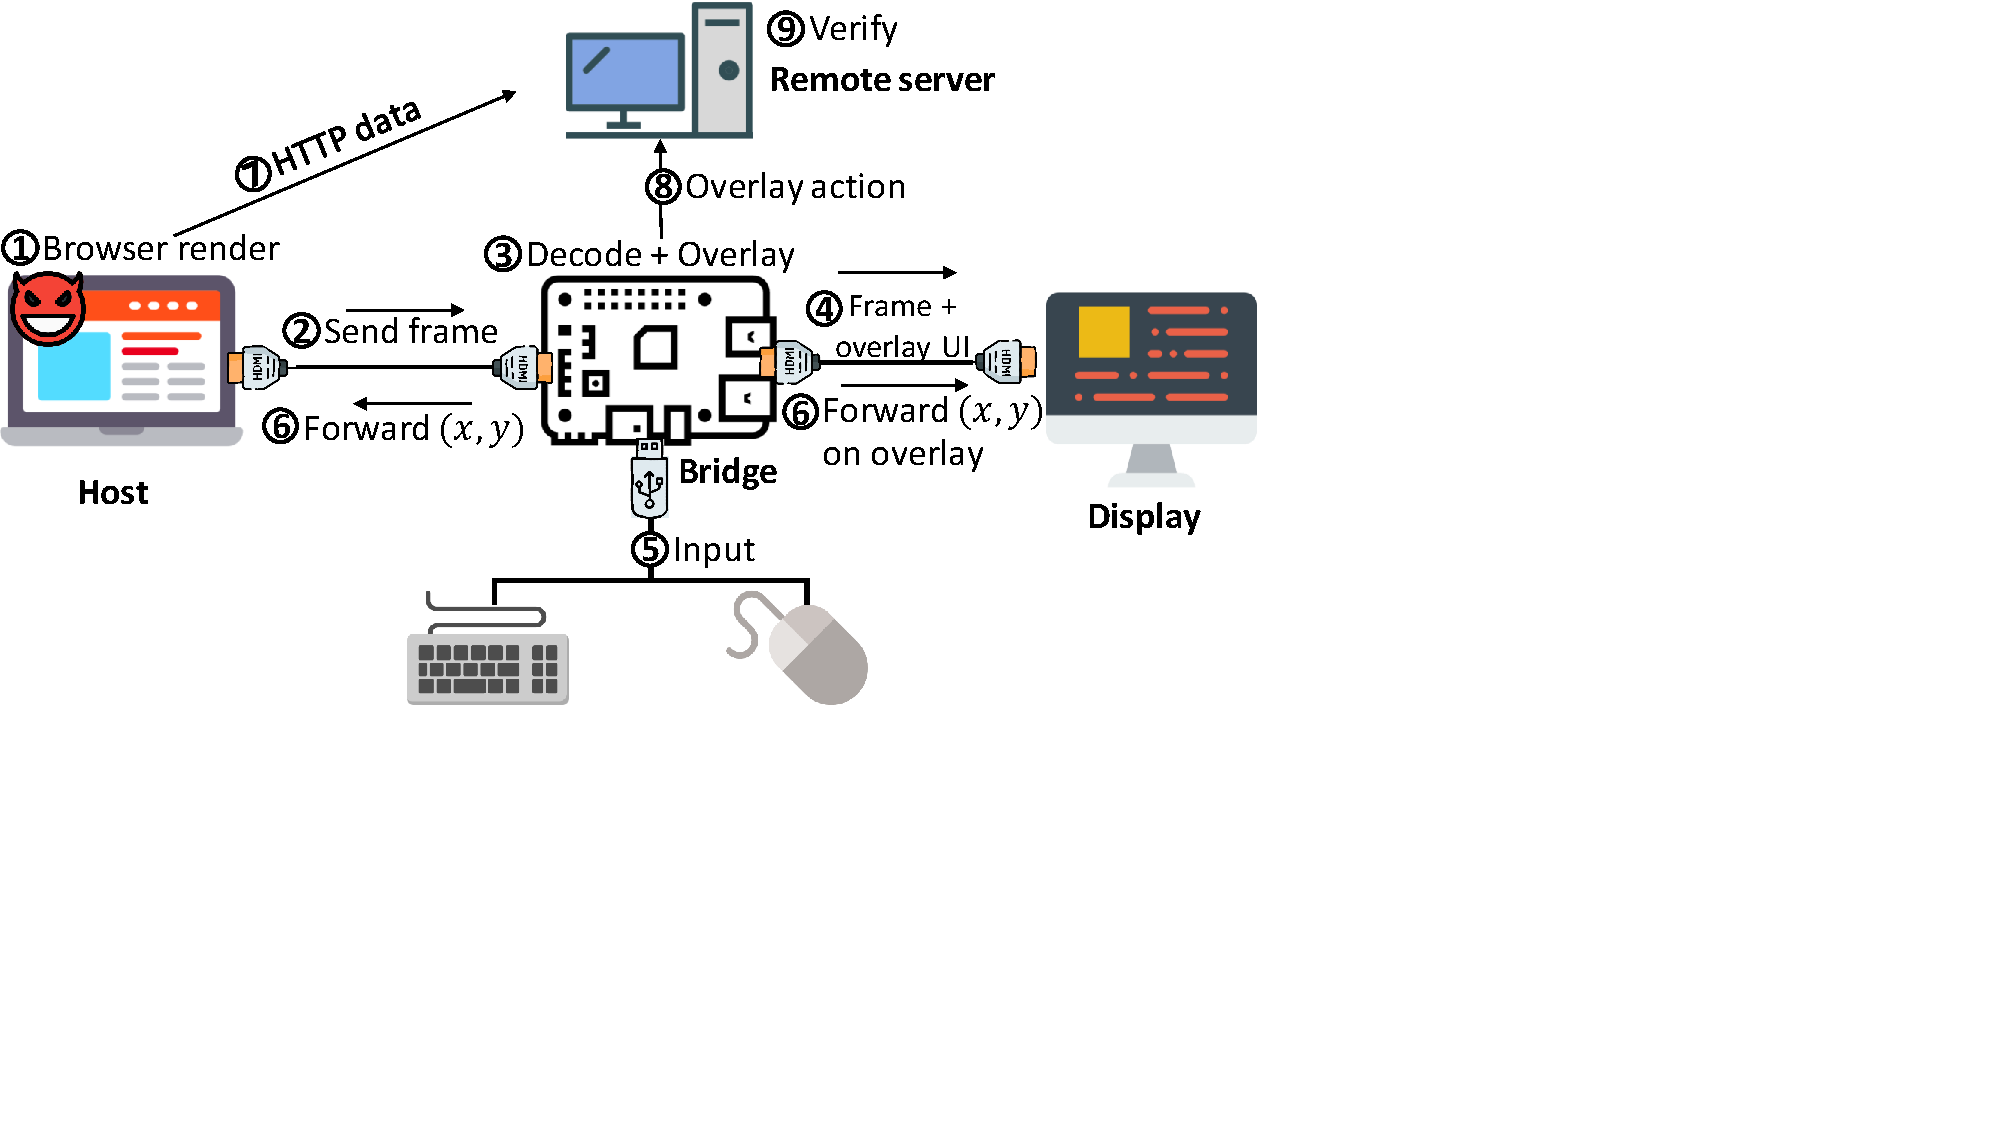
\includegraphics[trim={0 6cm 12cm 0}, clip, width=\linewidth]{systemDesign.pdf}
\caption{High level flow of \name}
\label{fig:systemDesign}
\centering
\end{figure}

In this section, we provide the technical details of \name that provides 
\subsection{System Components}
\label{sec:systemDesign:components}

Figure~\ref{fig:systemDesign} provides the overall system design of \name. The components of the systems are the following:

\begin{enumerate}
  \item \textbf{Host system.} The host system is completely compromised (hardware, OS and the installed applications) by the attacker.
  \item \textbf{\device.} The \device is connected to the input devices and sits between the host and the display. The \device is connected to the input devices over the \usb interface and connected to the host and the display over HDMI.
  \item \textbf{Input device.}
  \item \textbf{Display.}
  
\end{enumerate}

\subsection{Initialization} 
\label{sec''systemDesign:init}

There are two steps of initialization process: 

\begin{enumerate}
  \item\textbf{IO initialization.} The \device initializes the mouse by instructing the host system to move the mouse pointer to the top right corner (moving to the first right and then up for an arbitrarily large value). As the \device has access to the frames that are displayed on the screen, it can verify if the mouse pointer is at the top-right corner of the screen or not. Then it instructs the host OS to bring it to the center of the screen.
  
  \item\textbf{Network initialization.} The \device connects to the remote server using \webusb or \webbt, effectively using the host as an untrusted transport. The \device and the server establishes a secure channel with the public certificates that are distributed before-hand.
\end{enumerate}


\subsection{Key Establishment Protocol}
\label{sec:systemDesign:keyEstablishment}

\begin{figure}[t]
\centering
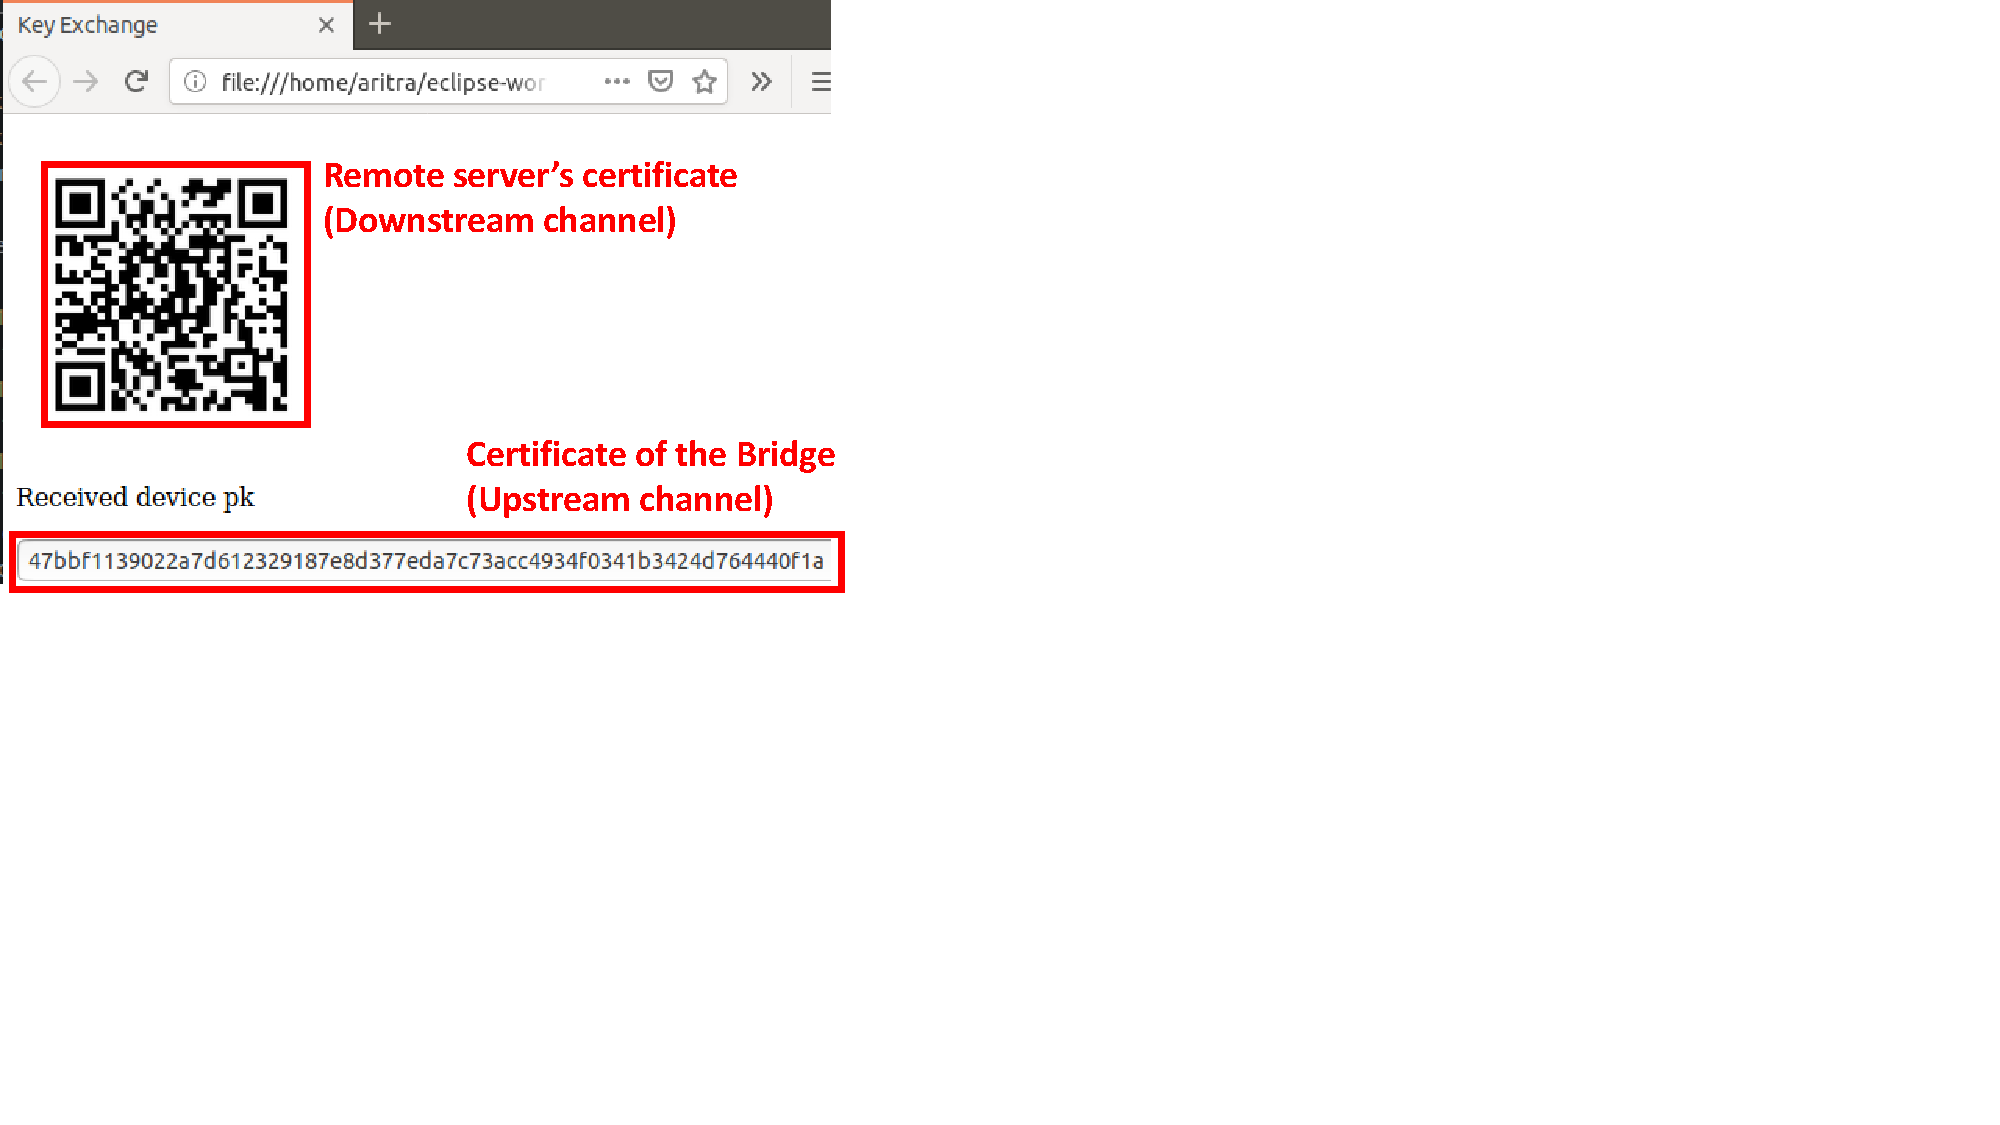
\includegraphics[trim={0 8cm 18cm 0}, clip, width=0.75\linewidth]{keyExchange.pdf}
\caption{\textbf{Key establishment.} A snapshot of the key exchange web page that is used to communicate the public certificates of the device and the remote server. This page only lasts for a few milliseconds, hence the page is practically invisible to the user.}
\label{fig:keyExchange}
\centering
\end{figure}


An instance of the key exchange mechanism of \name is illustrated in Figure~\ref{fig:keyExchange}. The flow of the key exchange mechanism is as the following:

\begin{enumerate}
  \item The web page shows a QR code that encodes the signed public key of the remote server. 
  \item The device captures the frames and looks for a QR code. As soon as the device finds one, the device decodes the QR code and verifies it.
  \item If the verification is successful, the device emulates itself as a keyboard device to the host system. The device then encodes its public certificate to hexadecimal and send it as a keystroke to the host.
  \item The JavaScript snippet looks for the keystrokes, and as soon as it gets a string of a specific length, it sends the key strokes to the remote server.  
\end{enumerate}

After this, both the device and the remote server have each other's public certificates. Using these certificates, they can then establish a shared secret by executing an authenticated Diffie-Hellman key exchange protocol.



\begin{figure*}[t]
\centering
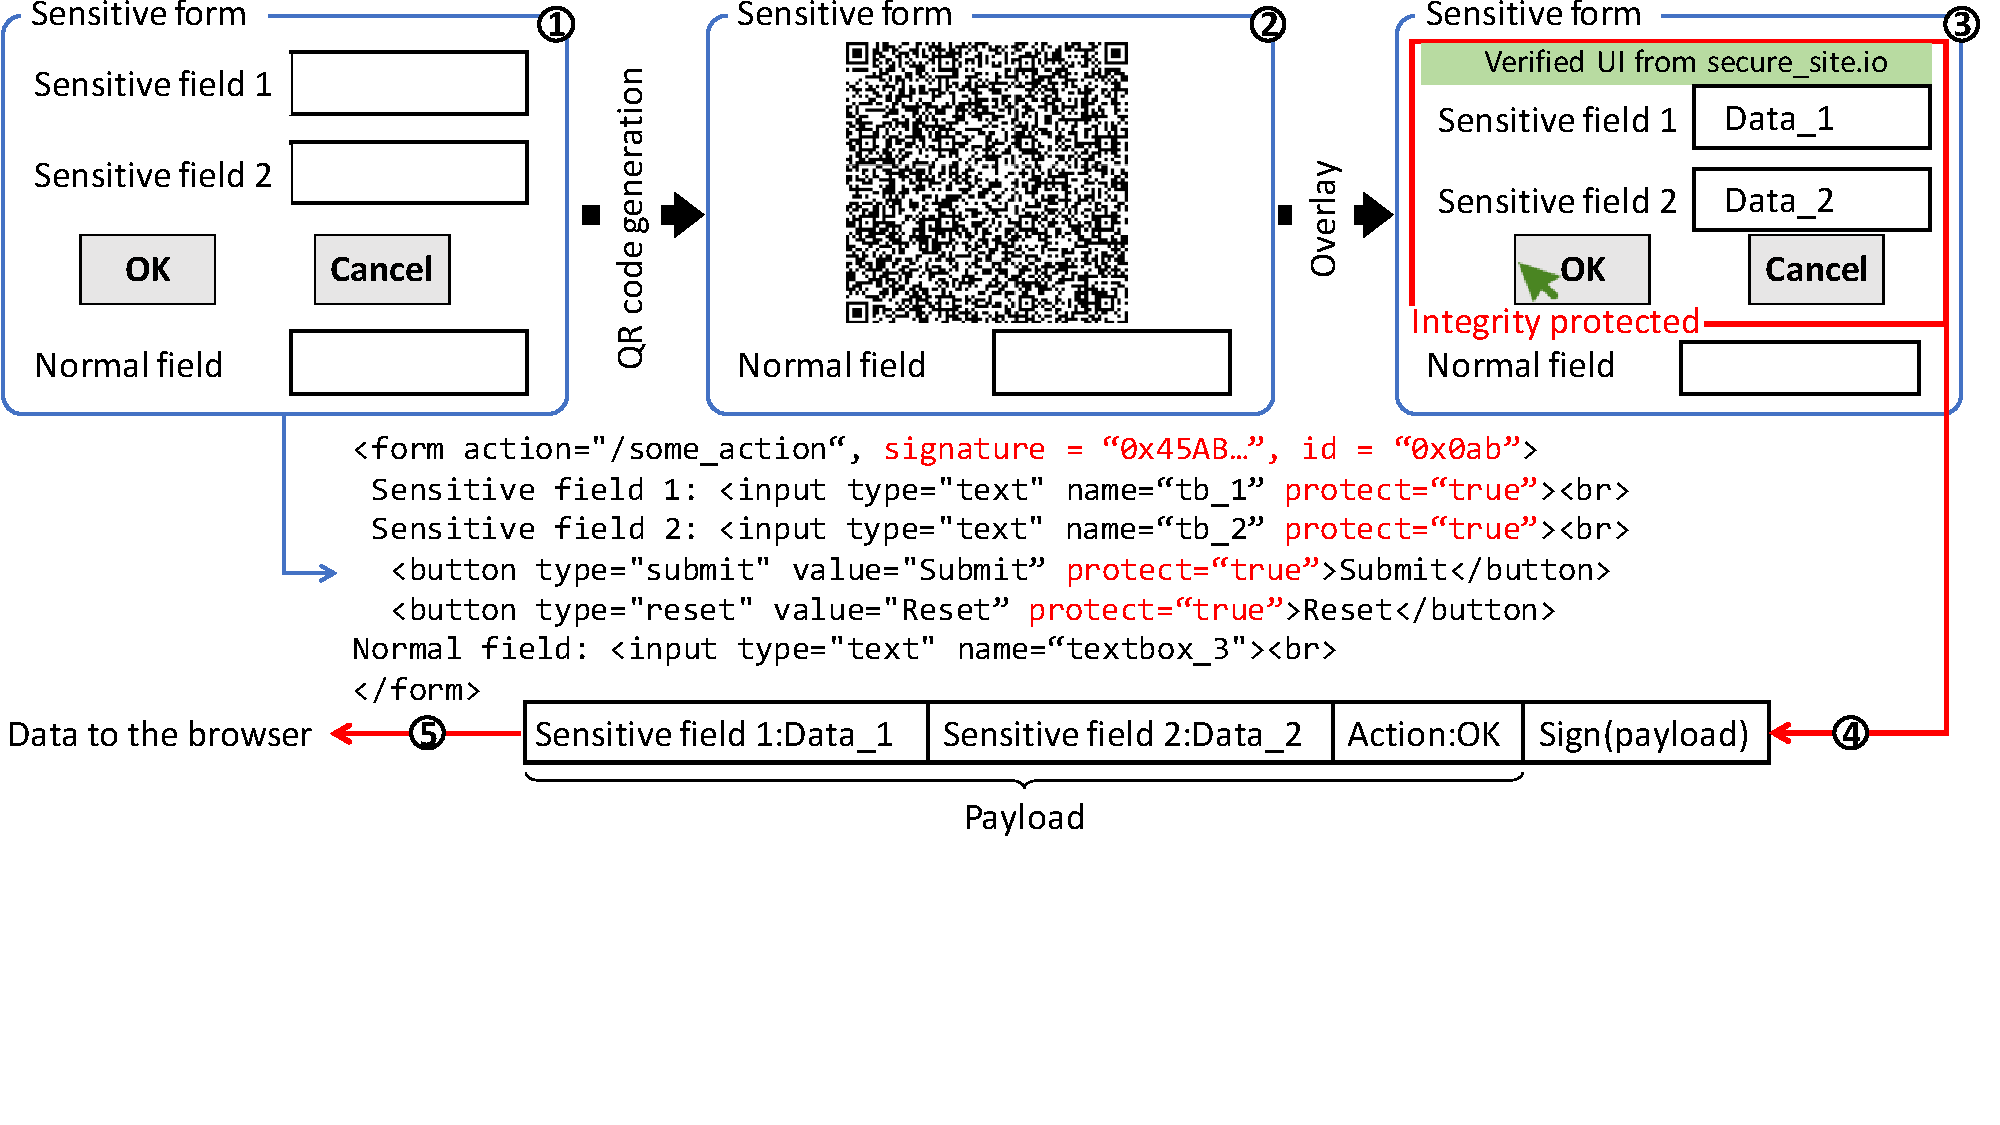
\includegraphics[trim={0 4cm 0 0}, clip, width=0.75\linewidth]{formTransform.pdf}
\caption{\textbf{Transformation of UI elements.} Automated transformation of the UI elements (\one) by the \name JavaScript snippets that detects the presence of the device. The corresponding \texttt{HTML} source shows the UI elements that requires integrity/privacy protection. These UI elements are transformed to a QR code (\two) that is decrypted and overplayed (\three) on the HDMI stream by the \device. Upon user's action on the overlayed UI elements, the device signs all the input data and send them to the remote server. Note that the intermediate QR code transformation (\two) is not visible by the user as it is decoded instantaneously by the device.}
\label{fig:transformation}
\end{figure*}

\subsection{Transformation of UI Elements for Proof-of-Action}
\label{sec:systemDesign:transformation}

After the establishment of the secure channel between the device and the remote server, the \name JS snippet that is served with the webpage transform the UI elements that requires protection. We illustrate the method of UI transformation in Figure~\ref{fig:transformation}. The entire process has three phases: \emph{transformation}, \emph{overlay}, and \emph{data transfer}.

\myparagraph{Transformation} The transformation of the web page UI elements are handled by the \name JavaScript snippet that is served from the remote server. UI elements that require integrity protection can be marked by the developers in the \html source. As illustrated in Figure~\ref{fig:transformation}, the \html UI elements that have additional attribute \texttt{protect=``true''} requires integrity protection from the \device. The transformation phase is between \one and \two in Figure~\ref{fig:transformation} where the \name JavaScript snippet transforms the UI elements to a UI specification language in a QR code that can be interpreted by the \device. The UI specification corresponding to the \html source (in Figure~\ref{fig:transformation}) is provided in Specification~\ref{snippet:UISpecification}.


\lstset{language=JSON, frame=tb, caption=\textbf{Protected UI specification language.} The UI specification shows the JSON formatted UI specification that is encoded into a QR code. The specification is generated from the \html source that are tagged as protected from the developers. The example specification is generated from the \html source that is provided in corresponding UI in Figure~\ref{fig:transformation}. , label = snippet:UISpecification, firstnumber =1}
\begin{figure}[t]
\begin{lstlisting}[mathescape=true]
{ "formId": "form1",
  "formName": "form1",
  "ui": [{ "id":"textbox\_1",
     "type":"textbox",
     "label":"Sensitive field 1",
     "text":"secret data 1"},
   { "id":"textbox_2",
     "type":"textbox",
     "label":"Sensitive field 2",
     "text":"secret data 2"},
   {"id":"OK_button",
     "type":"button",
     "trigger":"true",
     "label":"OK"},    
   {"id":"Cancel_button",
     "type":"button",
     "trigger":"false",
     "label":"Cancel"}]}
\end{lstlisting}
\end{figure}



\myparagraph{Overlay} Overlay is the next phase where the QR code that embeds the UI specification is interpreted by the \device and overlaid on the HDMI stream. The overlay faithfully recreates the UI to prevent any alteration in the user experience. The \device overlay is depicted in \three in Figure~\ref{fig:transformation}. The \device come with a small interpreter routine that converts the UI specifications to bitmaps that are then overlaid on the HDMI stream. 

\myparagraph{Data transfer} After the UI elements are correctly overlaid on the screen, the users can interact with the elements as if there is no alternation. The \device understands the semantics of all the generated UI elements, such as when a user selects a text box and types on her keyboard, the \device intercepts all the keyboard strokes and overlays the characters on the UI. When the user clicks on the \texttt{OK} button on the overlay, the device gathers all the intercepted keyboard and mouse events, signs them and send them to the remote server.  


\begin{figure}[t]
\centering
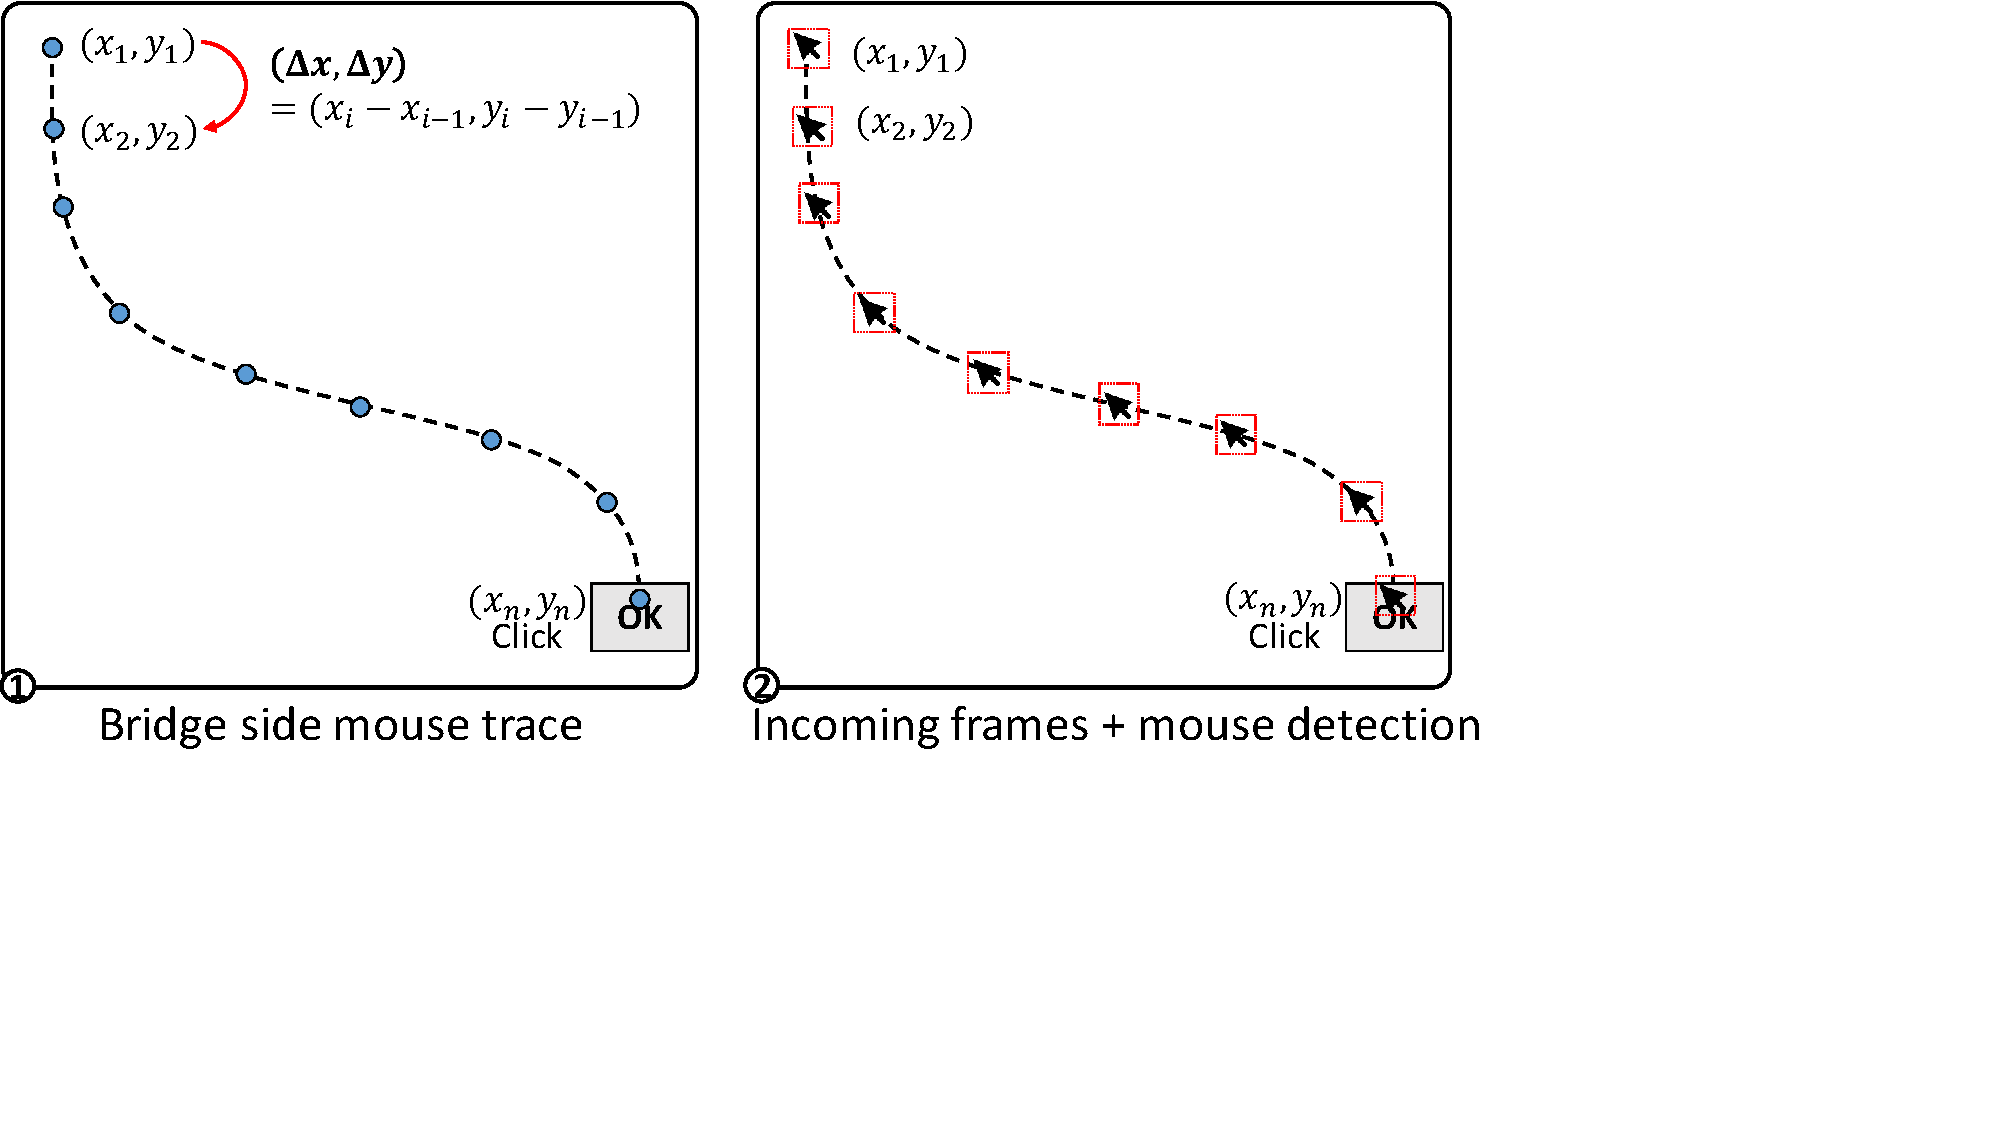
\includegraphics[trim={0 5.8cm 8cm 0}, clip, width=\linewidth]{mouseAnalysis.pdf}
\caption{\textbf{Proof-of-pointer.} The figure shows the high-level procedure of proof-of-pointer. The device knows the initial pointer position by sending a high mouse value to the host that puts the pointer on a specific corner $(x_0, y_0)$. \one The \device captures the raw mouse events ($\Delta x, \Delta y$) from the mouse that is attached to the \device. \two The \device captures the frames from the HDMI channel and checks into the designated pixel position $(x_i + \Delta x, y_i + \Delta y)$ if there exists a pointer.}
\label{fig:mouseAnalysis}
\centering
\end{figure}

\subsection{Analysis of HDMI Frames for Proof-of-pointer}
\label{sec:systemDesign:analysis}

The crucial property that \name provides is the user input integrity that combines both keyboard and mouse input. The integrity of the mouser input is nontrivial as one needs to know what the user sees on the screen. \name achieves this by intercepting the HDMI frames from the host system. The \device sits between the host and the display device (the monitor) and captures the frame to extract the cursor context. We call this property as the \emph{proof-of-pointer} where the \device generates the proof of the traces of the pointer. 

Figure~\ref{fig:mouseAnalysis} illustrates the high-level idea of the host system's HDMI frame analysis. To match the mouse polling rate with the display frame rate, the \device only queries the input device with the frequency of $60$ Hz. We assume that over the HDMI channel the host system sends frames at the rate of $60$ fps. The analysis works like the following. We define mouse movement as the time series $(x,y)$ co-ordinates $\{(x_1,y_1), (x_2, y_2), \ldots, (x_n,y_n)\}$ from time $\{t_1, t_2, \ldots, t_n\}$. Assume that the frames coming from the host system to the \device are: $\{f_1, f_2, \ldots, f_n\}$. In time $t_i$, the \device looks into the frame $f_i$ and draws a square centered at $(x_i, y_i)$ with sides of length $X$ (enough to cover a mouse cursor). Then the \device checks if there exists a mouse inside this square or not. In case there exists a mouse cursor, the \device allows further user interactions otherwise it stops all the communications and shows an error on display.



\subsection{Committing User Input}
\label{sec:systemDesign:commit}

When the user finishes providing her input over the input device (mouse and keyboard), the \device commits these values to the remote server. The commitment is executed by providing the signed input values to the remote server. The commitment procedure is illustrated in Figure~\ref{fig:transformation}. The commitment has two phases: \emph{record} and \emph{commit}.

\myparagraph{Record} When user provides any information on the rendered overlay UI elements (such as textbox, button, slider, radio button, etc.), the \device records that in a (key, value) pair where the key is the identifier of the UI element (\texttt{id} in Specification~\ref{snippet:UISpecification}) and the value is the user provided value. The \texttt{type} of the UI elements determine what information to record. For example, the \device records all the keystrokes when a textbox is selected, the value corresponding to the position of the slider is recorded when the user interacts with a slider, etc.

\myparagraph{Commit} In the commitment phase, the \device waits for the user to operate on a UI element which has a \texttt{trigger} capability. For example, in Specification~\ref{snippet:UISpecification}, the \texttt{OK} and the \texttt{cancel} buttons have an attribute \texttt{trigger}. This attribute can take either \texttt{true} (corresponding to \texttt{OK}) or \texttt{false} (corresponding to \texttt{Cancel}) value that denotes that the the button can submit the values that are provided by the user or abort the form altogether.  


\subsection{Main Protocol}
\label{sec:systemDesign:mainProtocol}

In Sections~\ref{sec:systemDesign:keyEstablishment}, \ref{sec:systemDesign:transformation}, \ref{sec:systemDesign:commit}, we explain the basic components of \name. Now in this Section, we provide the overall protocol/

The outline of the system is illustrated in Figure~\ref{fig:systemDesign}. The steps are the following:


\begin{enumerate}
  \item[\one], The user, provides input from her input device which is captured by the \device.
  \item[\two] The \device sends the mouse traces to the host over the \bluetooth interface.
  \item[\three] The host system draws the frames.
  \item[\four], The host, sends the drawn frames to the \device over HDMI interface.
  \item[\five] The host sends the \http request to the remote server that contains user input. 
  \item[\six] The remote server sends the UI information to the \device over the dedicated \tls channel between the \device and the remote server. The packet includes information such as the type of the UI, text that is expected on the UI, etc.
  \item[\seven] The \device analyzes the frames (from step \four) from the host using the UI information (step \six) received from the server. The analysis step is discussed in details in Section~\ref{sec:systemDesign:analysis}.
  \item[\eight] The \device sends the frames and the overlay derived from the analysis step to the display device.

\end{enumerate}



\begin{figure}[t]
\centering
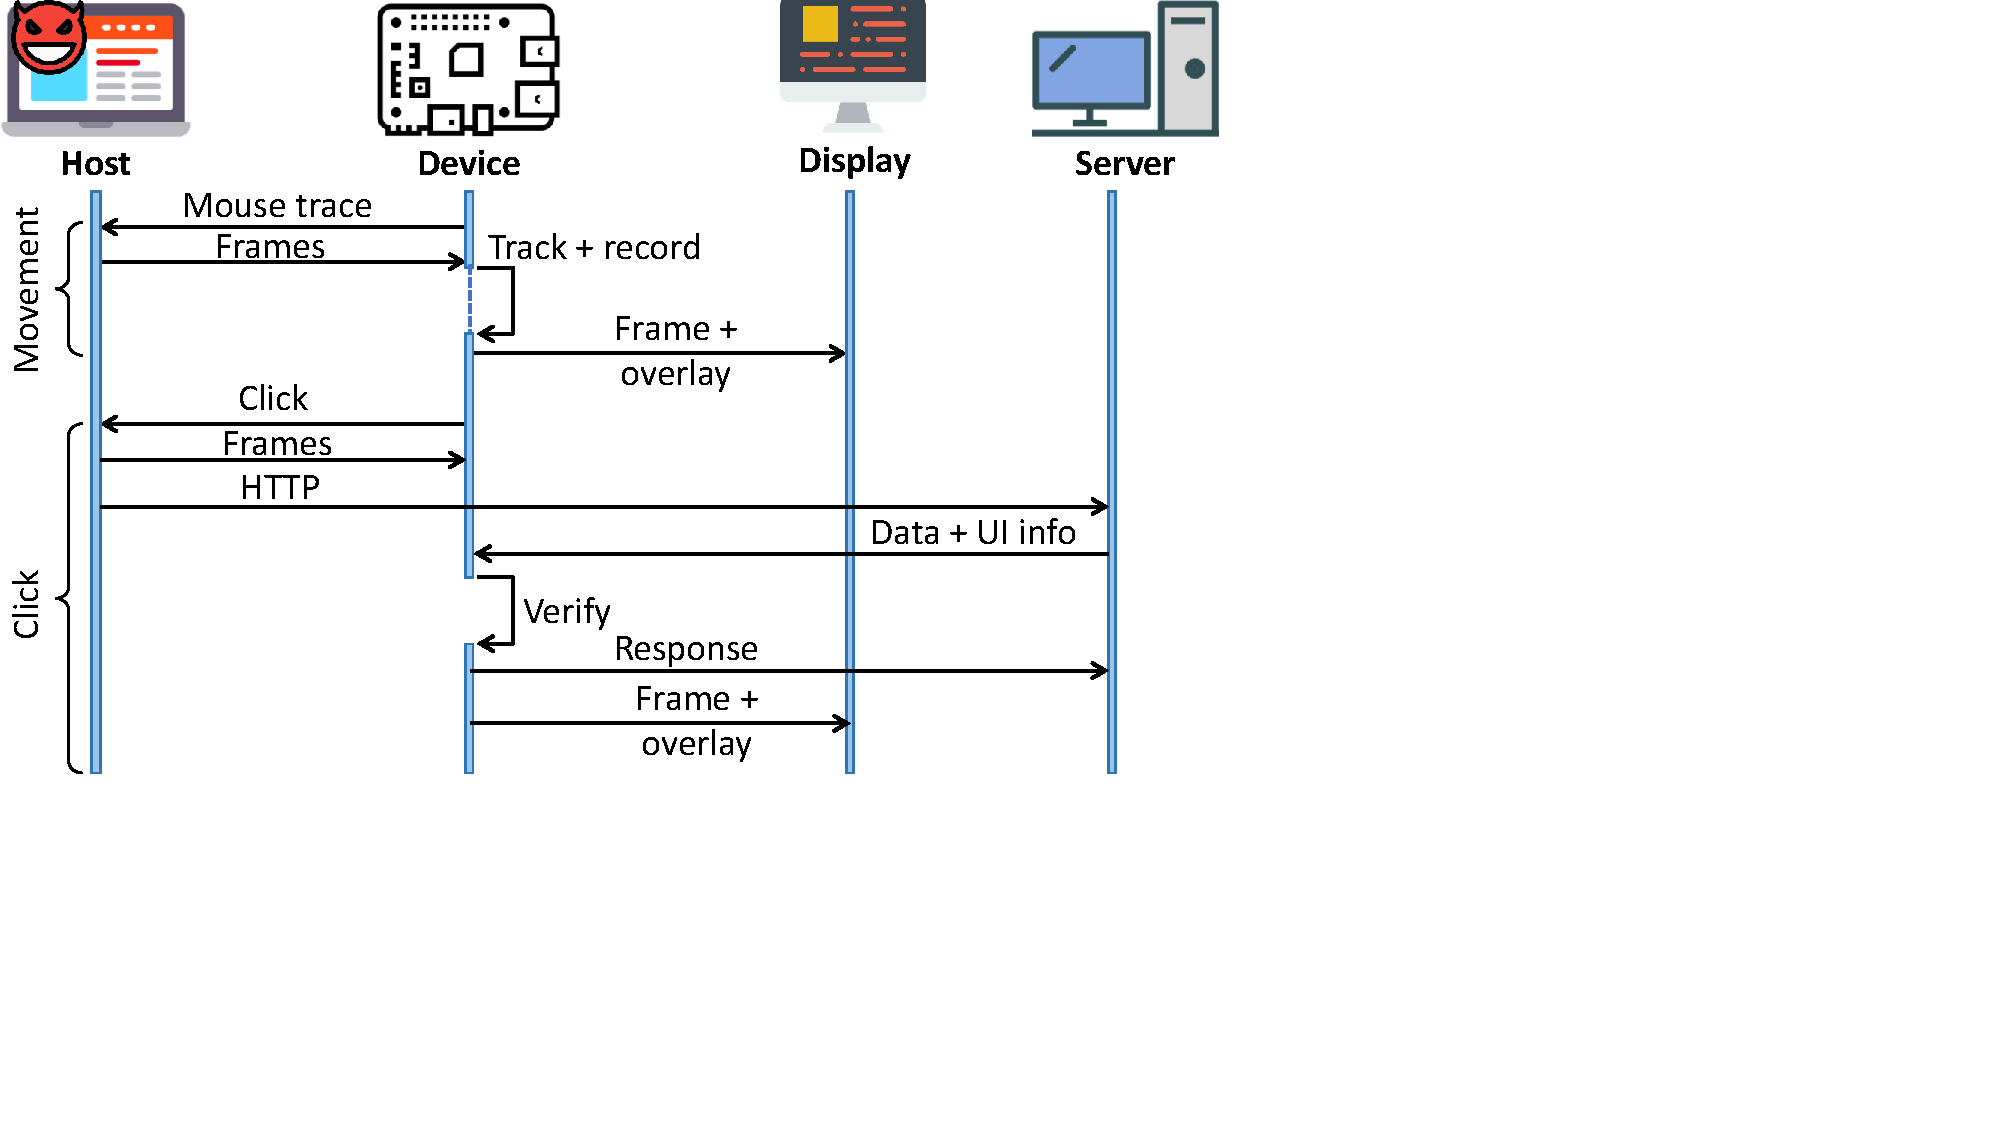
\includegraphics[trim={0 5.8cm 13cm 0}, clip, width=\linewidth]{flow.pdf}
\caption{Protocol}
\label{fig:protocol}
\end{figure}




\iffalse
\begin{figure}[t]
\centering
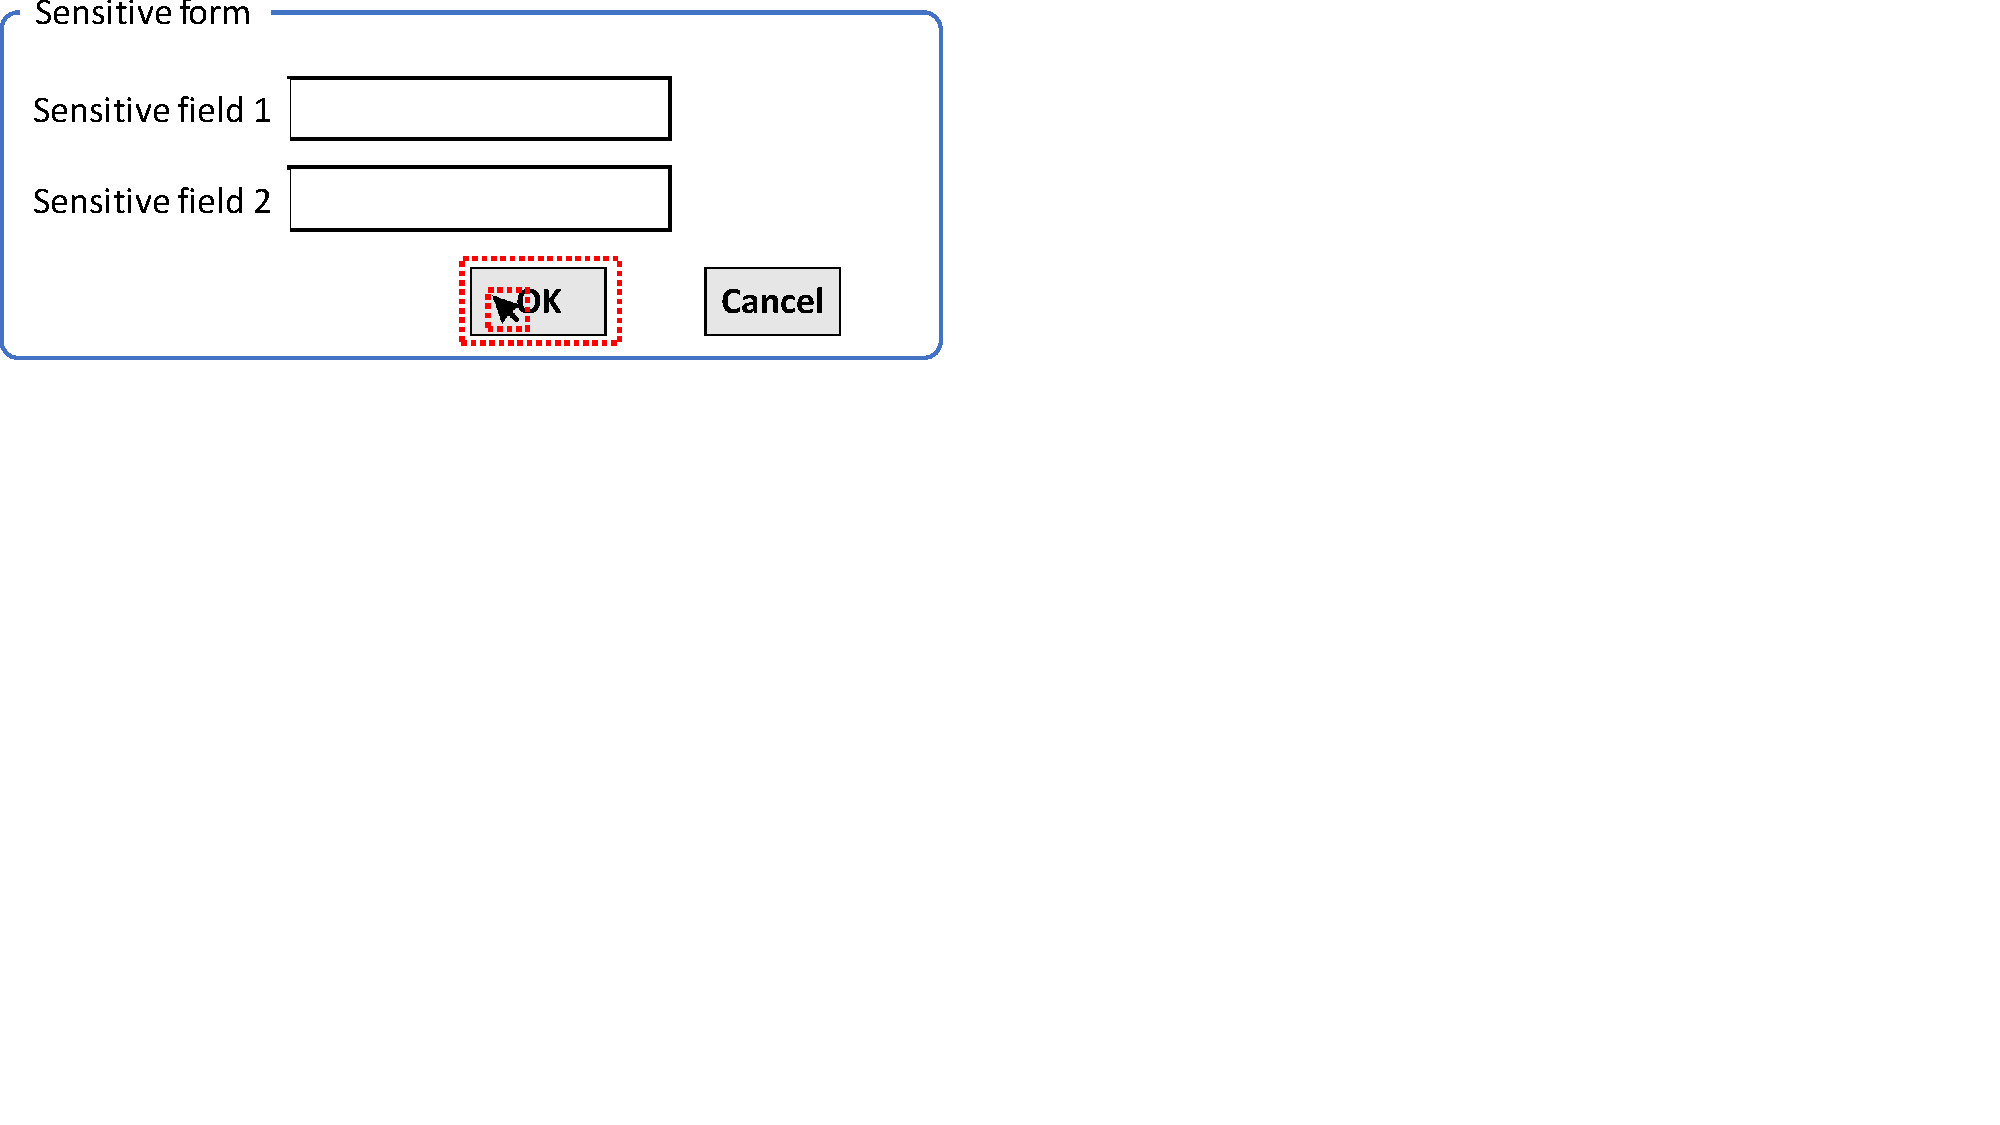
\includegraphics[trim={0 12cm 17cm 0}, clip, width=0.8\linewidth]{uiDetect.pdf}
\caption{Detection of the UI elements upon mouse click event in the incoming frame.}
\label{fig:uiDetect}
\centering
\end{figure}
\fi
% \begin{figure}
% \centering
% 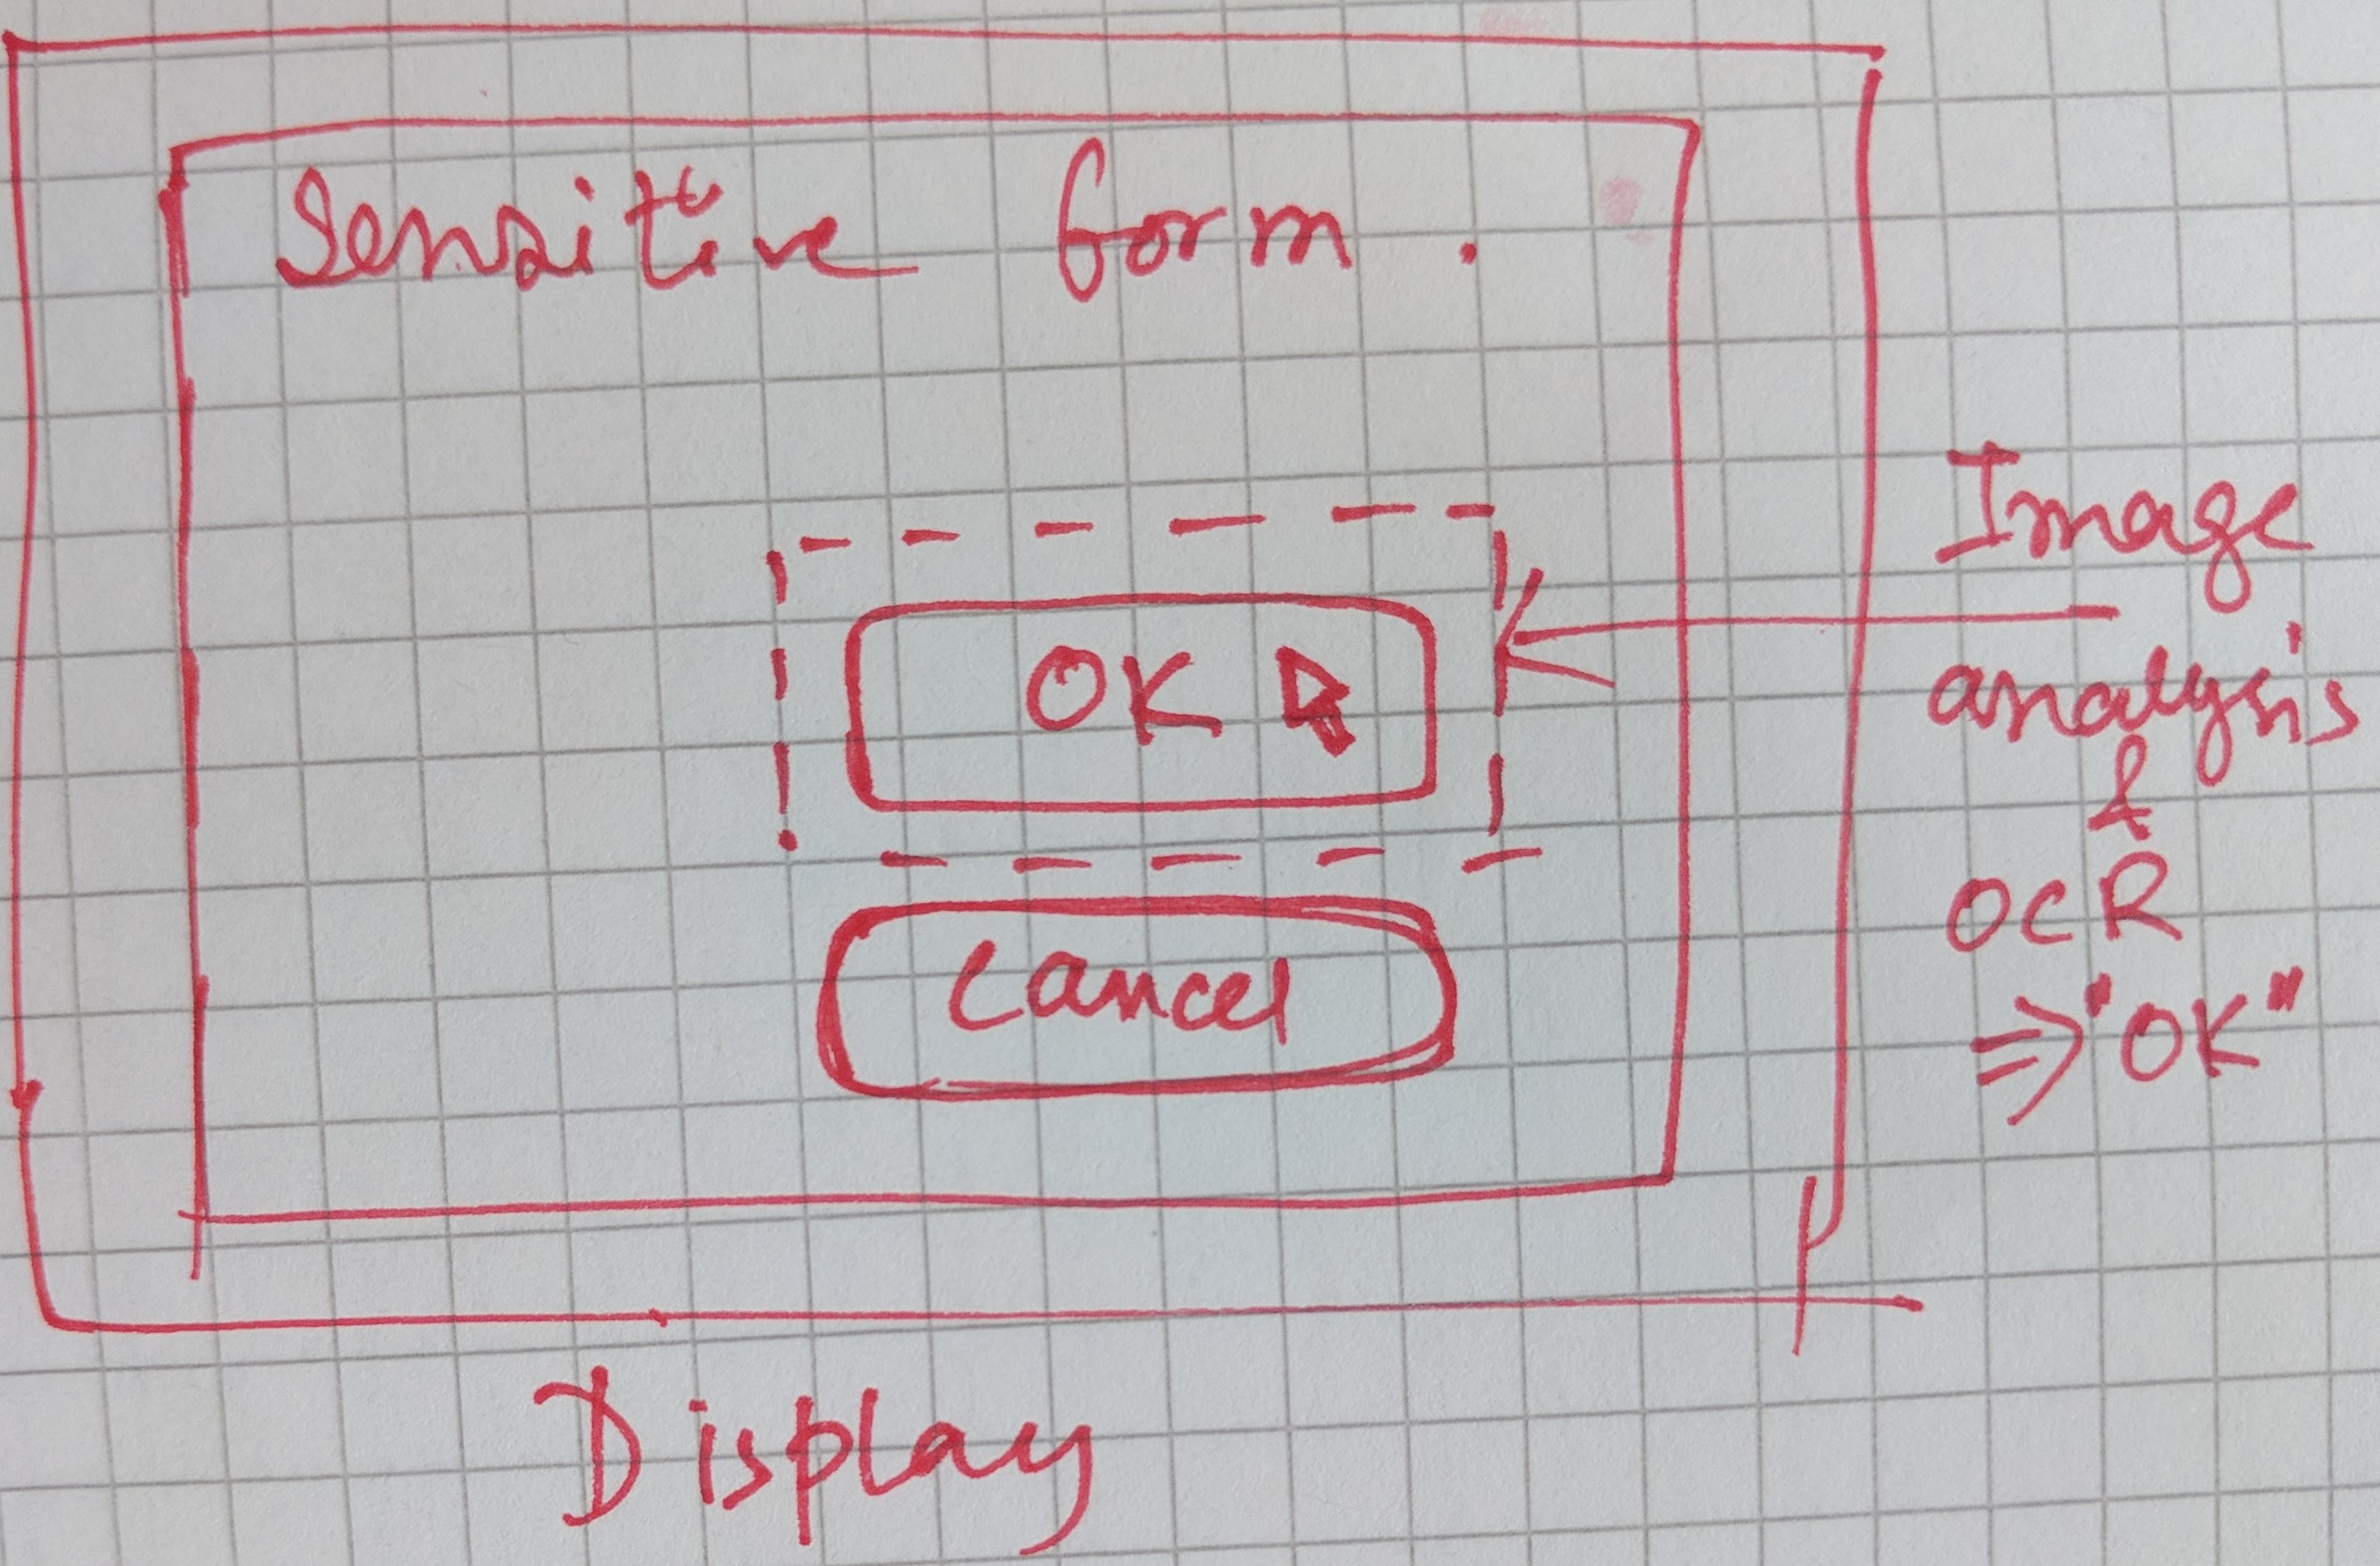
\includegraphics[width=\linewidth]{ui_detect.jpg}
% \caption{Detection of UI elements}
% \label{fig:uiDetect}
% \centering
% \end{figure}



\iffalse
\subsection{Detecting UI elements}
\label{sec:systemDesign:uiElements}

Detecting the UI elements triggers when the user clicks. The \device uses a square of $X$ square pixels around the mouse pointer and analyze the image. Figure~\ref{fig:uiDetect} illustrates an example of detecting the UI element from the captured frame. For example, if the user clicks on a button, the \device executes the image analysis on the part of the image to try to figure out if there is a button and parse the text. Additionally, the \device also sends the button text to the server. The server checks the data sent by the \device and the data received from the browser and compares them. In case there is a mismatch, the server notifies the \device and the \device overlays an error message on the screen. 
\fi

\begin{figure}[h]
\centering
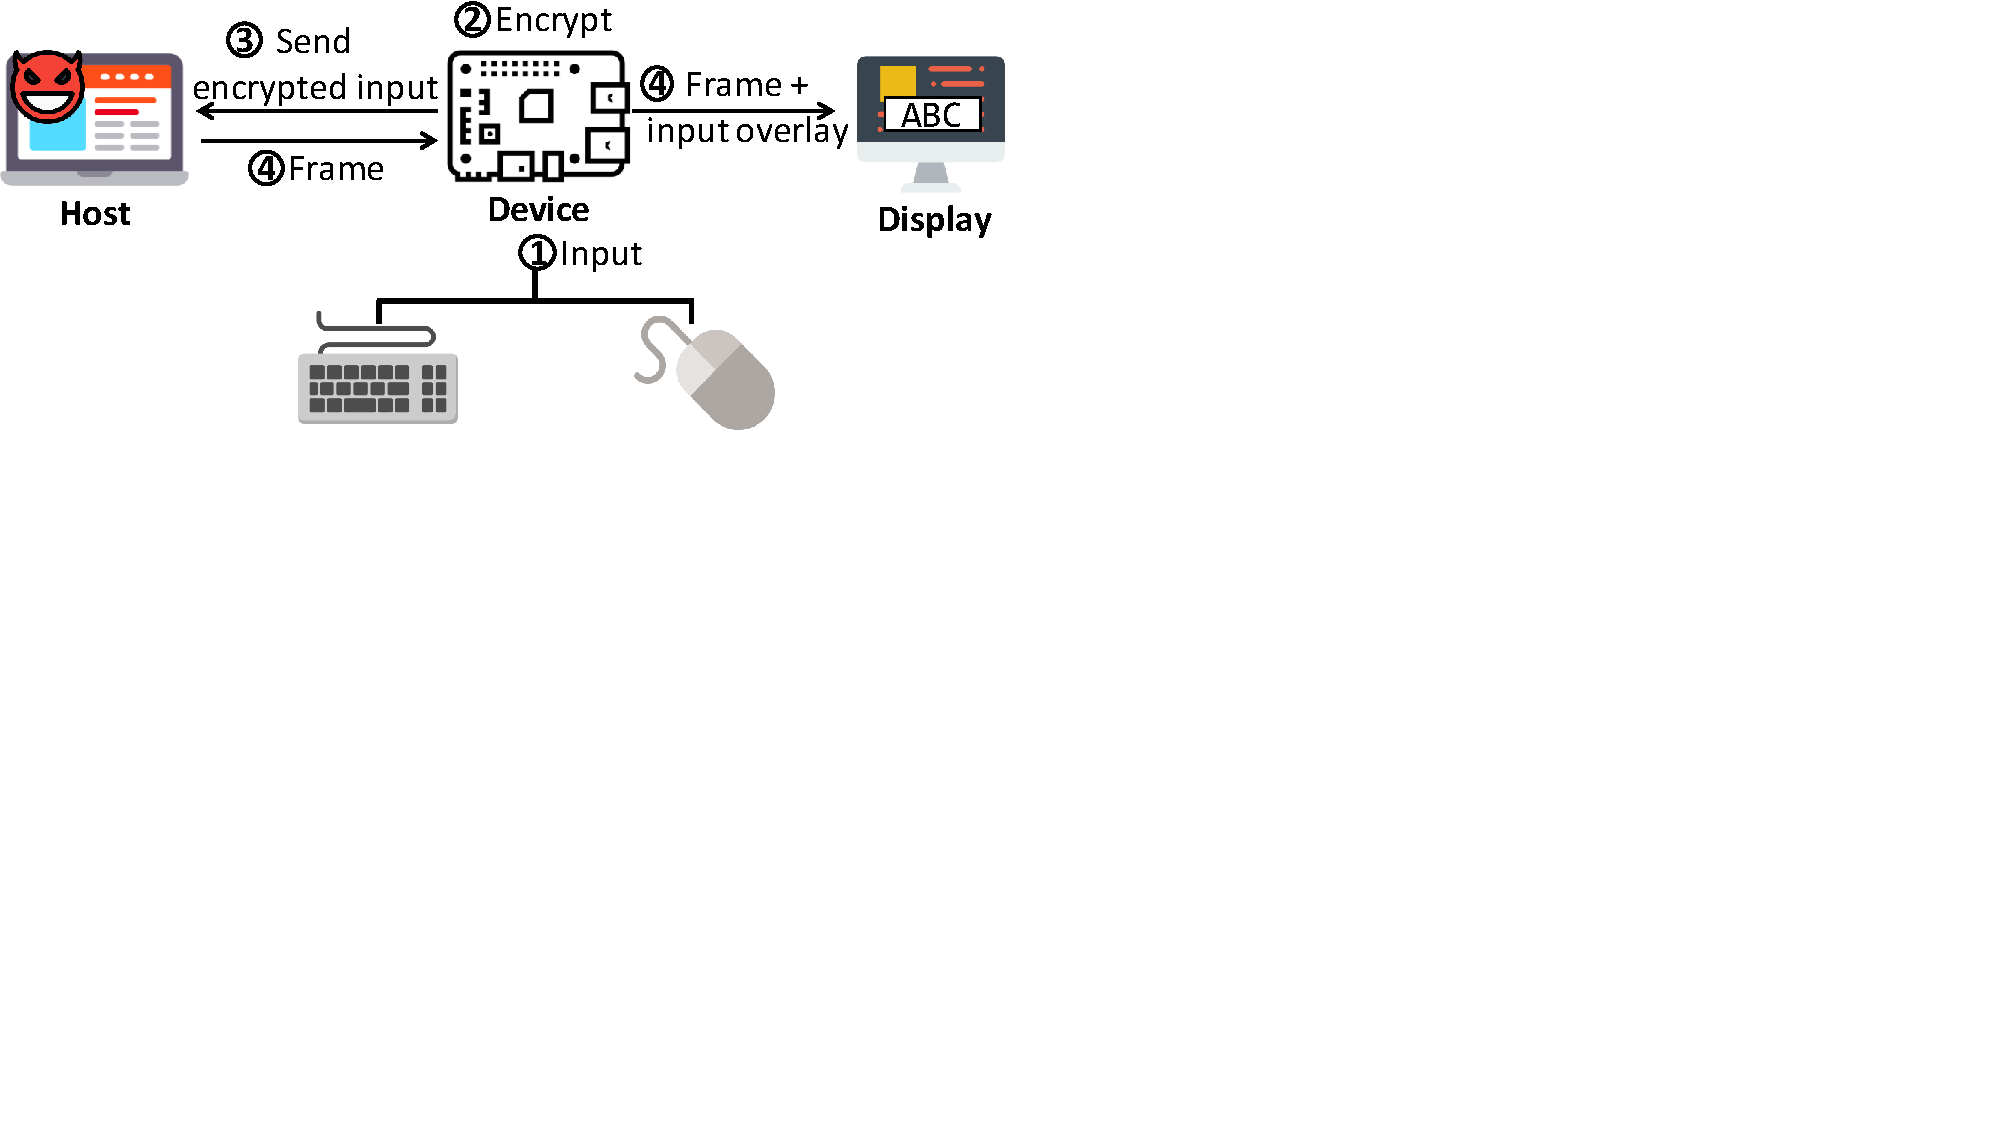
\includegraphics[trim={0 11cm 16.5cm 0}, clip, width=\linewidth]{inputPrivacy.pdf}
\caption{Input privacy}
\label{fig:inputPrivacy}
\centering
\end{figure}

